In this section, we will explain our findings of different buildings from the perspective of supply and demand analysis. We have used our previously described algorithm with the objective of finding $k-$best nearest buildings for booking a meeting room for different factors. We have completed the analysis for the following buildings where there is a high supply-demand problem:
\begin{itemize}
    \item Doug McDonell Building, Parkville (168) - Appendix Table \ref{appendix:doug_mr}
    \item 11 Barry St, Parkville (266) - Appendix Table \ref{appendix:barry_mr_table}
    \item Law Building, Parkville (106) - Appendix Table \ref{appendix:law_building_mr_table}
    \item David Penington Building, Parkville (102) - Appendix Table \ref{appendix:david_building_mr_table}
    \item FBE Building, Parkville (105) - Appendix Table \ref{appendix:fbe_building_mr_table}
    \item Medical Building, Parkville (181) - Appendix Table \ref{appendix:medical_building_mr_table}
    \item Elisabeth Murdoch Building, Southbank (860) - Appendix Table \ref{appendix:southbank_elisabeth_mr_table}
    \item Werribee Pathology Building, Werribee (416) - Appendix Table \ref{appendix:werribee_pathology_mr_table}
\end{itemize}

We will be summarising results for \texttt{ Doug McDonell Building}, \texttt{David Penington Building} and \texttt{Elisabeth Murdoch Building} as discussed in the below section.


\paragraph{Doug McDonell Building (Parkville Campus)}

As per our previous shown data analysis, this building is having the highest supply-demand problem as shown in the Figure \ref{fig:doug_mr_s_vs_d}. 

\begin{figure}[H]
\centering
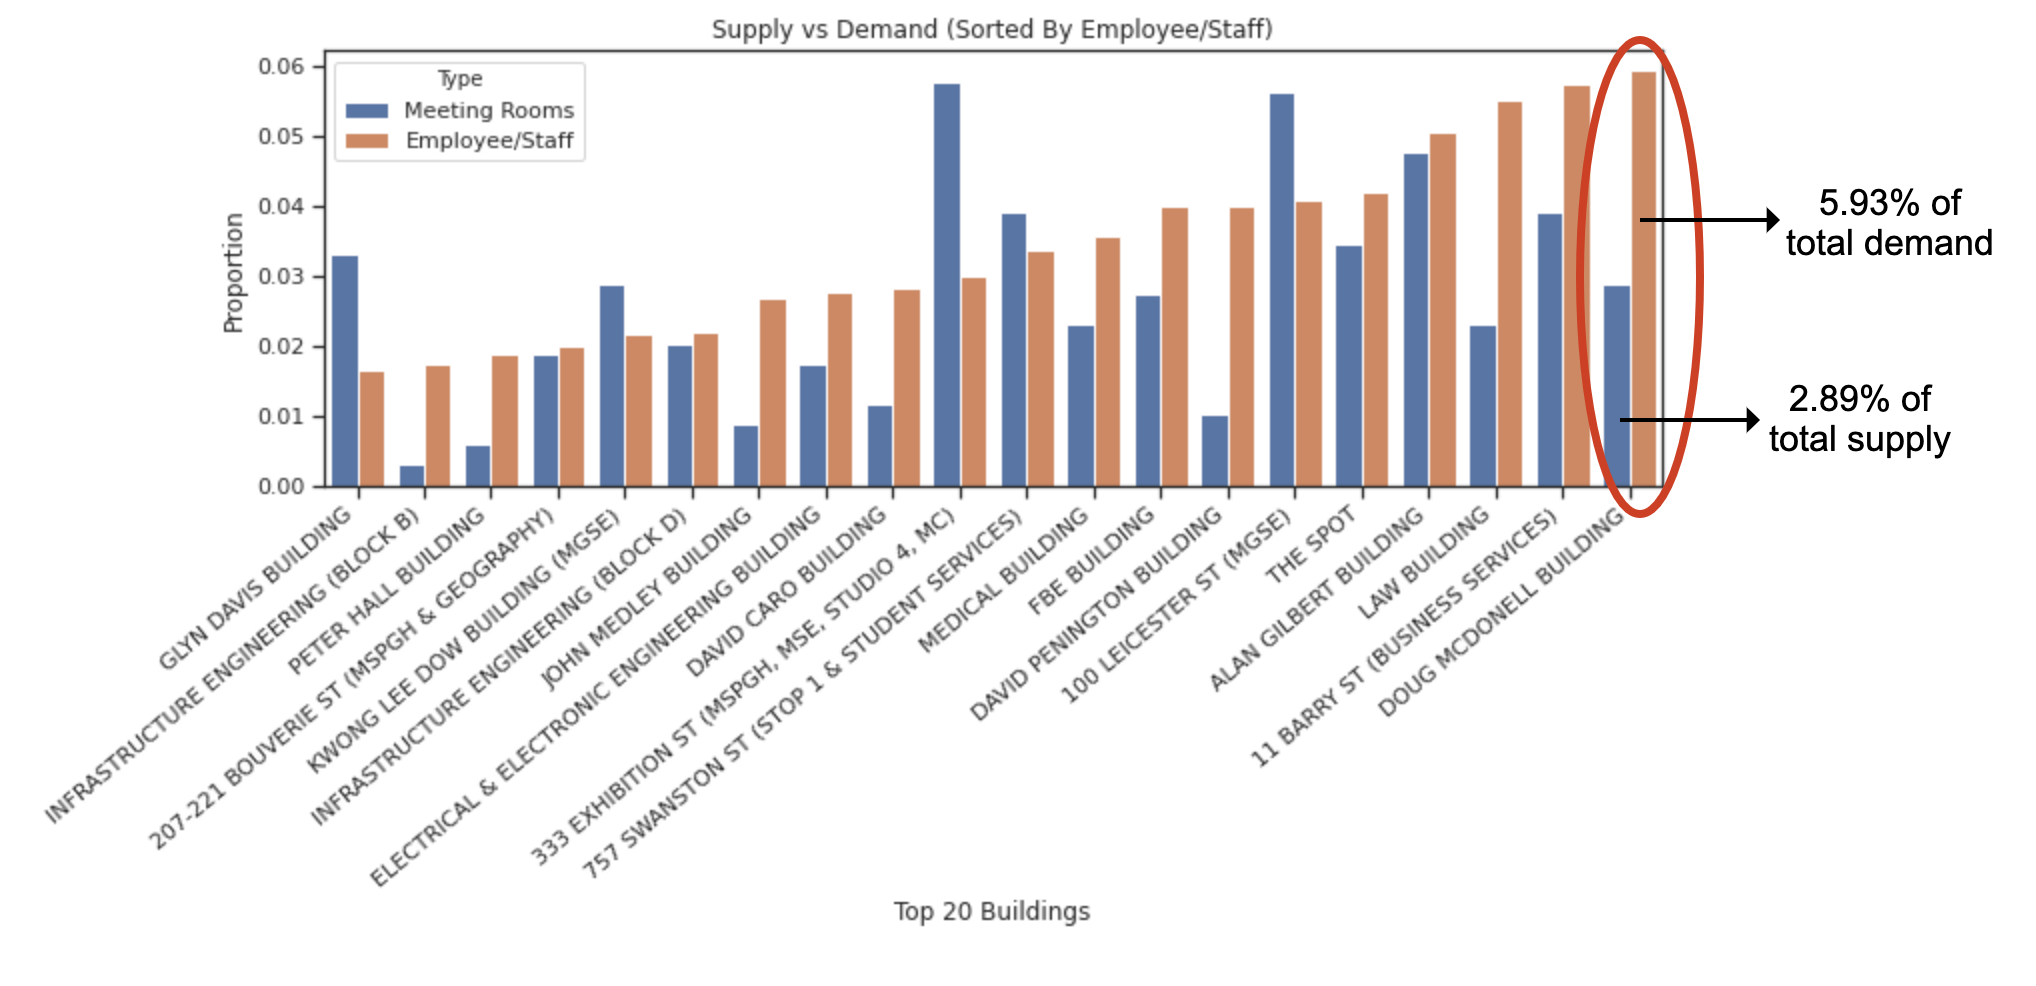
\includegraphics[width=10cm,keepaspectratio=true]{spatial-mr/doug-mr-results/doug_mr_s_vs_d.png}
\caption{Supply vs Demand Problem in Doug McDonell Building}
\label{fig:doug_mr_s_vs_d}
\end{figure}

As per the above plot, we can expect that there is a high chance that staff members are not able to find adequate meeting rooms in this building. Hence, we used our algorithm to find other best nearest buildings from Doug McDonell Building based on the different factors as interpreted below.

\begin{itemize}
    \item \textbf{Best nearby buildings with no preference:} As shown in the Appendix Table \ref{appendix:doug_mr}, a staff member needs to walk at least \texttt{302 metres} (Budget) from Doug McDonell Building to get rewarding buildings with an adequate supply of meeting rooms. We also suggest a relaxing budget ($\delta$) of \texttt{96 metres} so that employee doesn't miss out a high supply providing building. Using these constraints, we suggest \texttt{University Health Services Building (385)} as the most rewarding building with the cost of \texttt{432 metres} as shown in the Figure \ref{fig:doug-mr-no-factors}.
    
\begin{figure}[H]
\begin{subfigure}{.5\textwidth}
\centering
  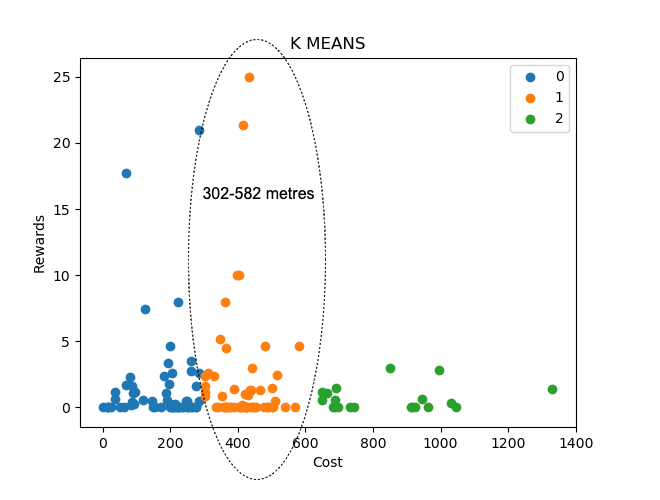
\includegraphics[width=8cm]{resources/images/spatial-mr/doug-mr-results/clusters_reward.png}
\end{subfigure}%
\begin{subfigure}{.5\textwidth}
  \centering
  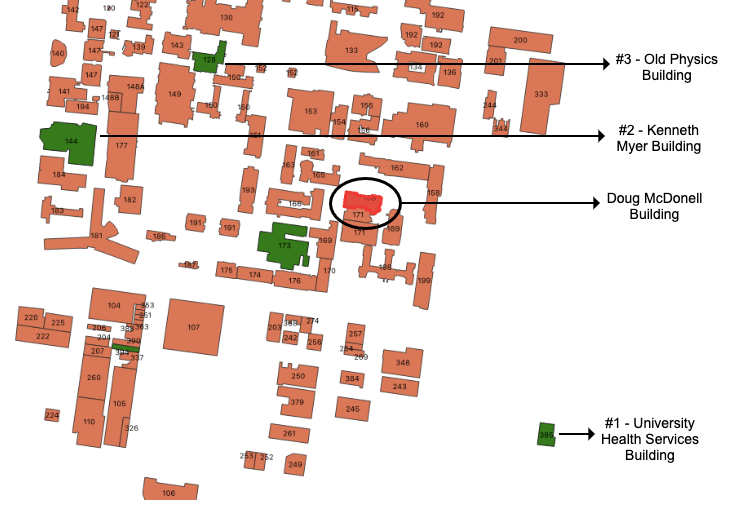
\includegraphics[width=8cm]{resources/images/spatial-mr/doug-mr-results/mr_spatial_view.png}
\end{subfigure}
\caption{Best rewarding cluster (left) and 3 most optimal buildings from Doug McDonell (right)}
\label{fig:doug-mr-no-factors}
\end{figure}

\item \textbf{Best nearby buildings under COVID-19 Strict Lockdown:} As shown in the Appendix Table \ref{appendix:doug_mr} with COVID-19 strict factor, a staff member should be willing to walk at least \texttt{648 metres} (Budget) from Doug McDonell Building to get very high rewarding buildings under COVID-19 lockdown with the relaxing budget($\delta$) of at least \texttt{16 metres}. Using these constraints, we suggest \texttt{The Spot building (110)} as the most rewarding building with the cost of \texttt{501 metres} followed by \texttt{Alan Gilbert building (104)} with \texttt{353 metres}.

% \item \textbf{Best nearby buildings with High Capacity:} As shown in the Appendix Table \ref{appendix:doug_mr} with high capacity factor, a staff member can easily find high supply of meeting rooms providing buildings from Doug McDonell building within the budget of \texttt{286 metres}. Using these constraints, we again suggest \texttt{Old Physics Buildings (128)} as the most rewarding building with the cost of \texttt{286 metres} followed by \texttt{Old Engineering School (173)} with \texttt{68 metres} and \texttt{Baillieu Library (177)} with \texttt{346 metres}.

\item \textbf{Best nearby buildings with other factors:} In the appendix Table \ref{appendix:doug_mr}, we have also shown other factors such as finding meeting rooms with equipment, excellent conditions and easy availability with their budgets and relaxing budgets. Using those constraints, we suggest that \texttt{Kenneth Myer Building (173) - 414 metres} is the most rewarding building for meeting rooms with equipment and finding meeting rooms in excellent condition. \texttt{University Health Services Building (385) - 432 metres} is the most rewarding building for finding easily available meeting rooms.

The results of some of the above-discussed factors are summarized below using clustering diagrams.

\begin{figure}[H]
\centering
\begin{subfigure}[b]{0.30\textwidth}
  \centering
  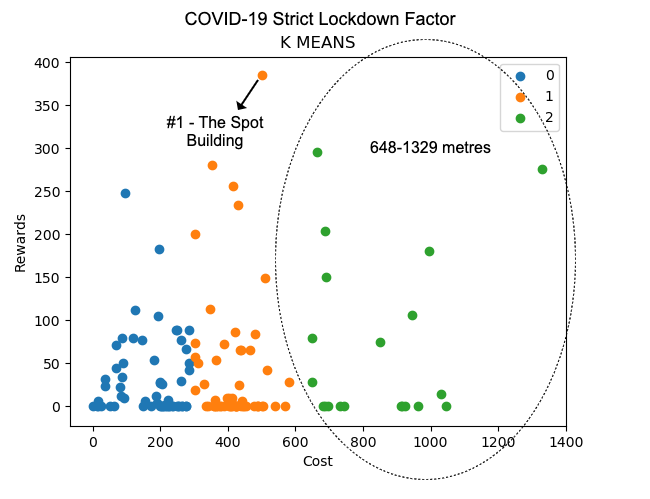
\includegraphics[width=5.5cm,keepaspectratio=true]{resources/images/spatial-mr/doug-mr-results/clusters_reward_covid_19.png}
\end{subfigure}
\begin{subfigure}[b]{0.30\textwidth}
  \centering
  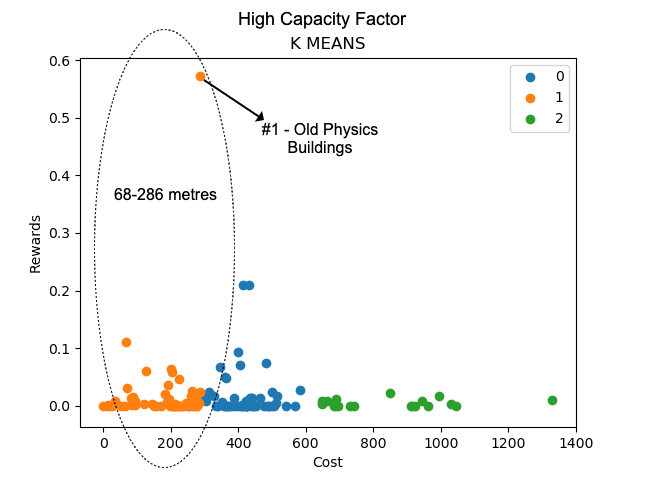
\includegraphics[width=5.5cm,keepaspectratio=true]{resources/images/spatial-mr/doug-mr-results/clusters_reward_high_cap.png}
\end{subfigure}
\begin{subfigure}[b]{0.30\textwidth}
  \centering
  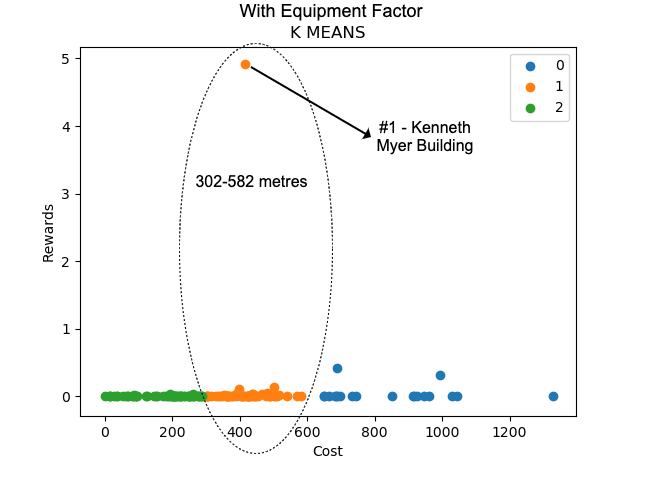
\includegraphics[width=5.5cm,keepaspectratio=true]{resources/images/spatial-mr/doug-mr-results/clusters_reward_with_eqps.png}
\end{subfigure}
\caption{Best rewarding clusters of nearby buildings from Doug McDonell based on different factors}
\label{fig:doug-mr-other-factors}
\end{figure}
    
\end{itemize}

% \paragraph{11 Barry St Building (Parkville Campus)}

% \begin{figure}[H]
% \centering
% 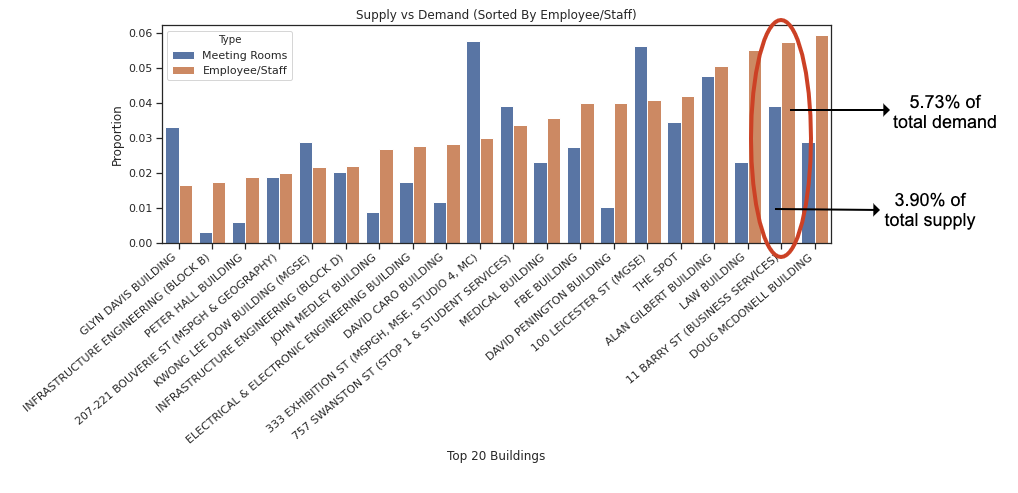
\includegraphics[width=10cm,keepaspectratio=true]{resources/images/spatial-mr/barry-mr/11_barry_st_01.png}
% \caption{Supply vs Demand Problem in 11 Barry St Building}
% \label{fig:barry_mr_s_vs_d}
% \end{figure}

% \begin{itemize}
%     \item \textbf{Best nearby buildings with no preference:}
    
%     \begin{figure}[H]
% \begin{subfigure}{.5\textwidth}
% \centering
%   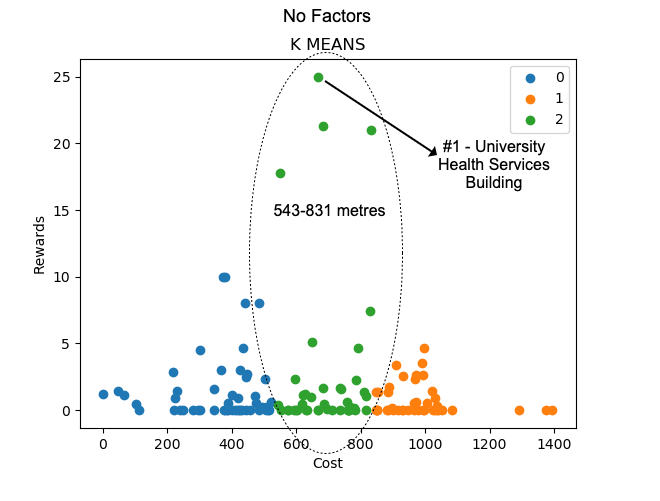
\includegraphics[width=8cm]{resources/images/spatial-mr/barry-mr/11_barry_st_03.png}
% \end{subfigure}%
% \begin{subfigure}{.5\textwidth}
%   \centering
%   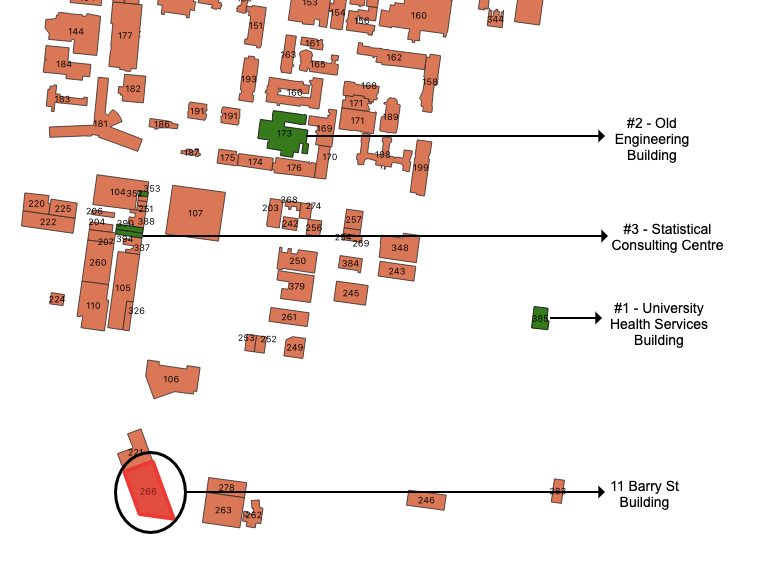
\includegraphics[width=8cm]{resources/images/spatial-mr/barry-mr/11_barry_st_02.png}
% \end{subfigure}
% \caption{Best rewarding cluster (left) and 3 most optimal buildings from 11 Barry St (right)}
% \label{fig:barry-mr-no-factors}
% \end{figure}

% \item \textbf{Best nearby buildings with equipment:}

% \item \textbf{Best nearby buildings with excellent room conditions:}

% \item \textbf{Best nearby buildings with other factors:}

% \end{itemize}

% The results of some of the above discussed factors are summarized below using clustering diagrams.

% \begin{figure}[H]
% \centering
% \begin{subfigure}[b]{0.30\textwidth}
%   \centering
%   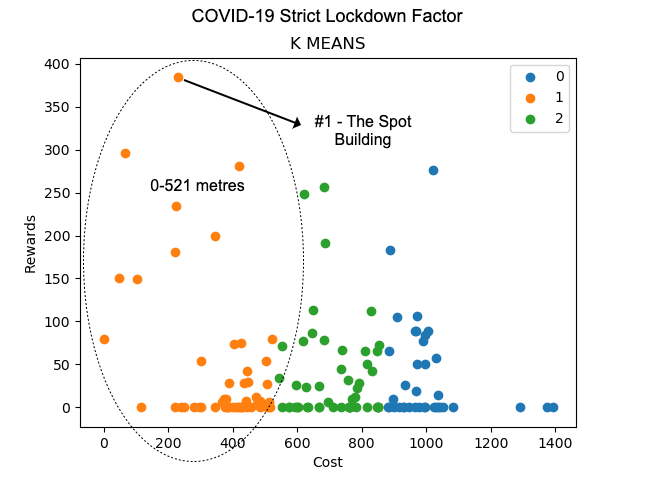
\includegraphics[width=5.5cm,keepaspectratio=true]{resources/images/spatial-mr/barry-mr/11_barry_st_04.png}
% \end{subfigure}
% \begin{subfigure}[b]{0.30\textwidth}
%   \centering
%   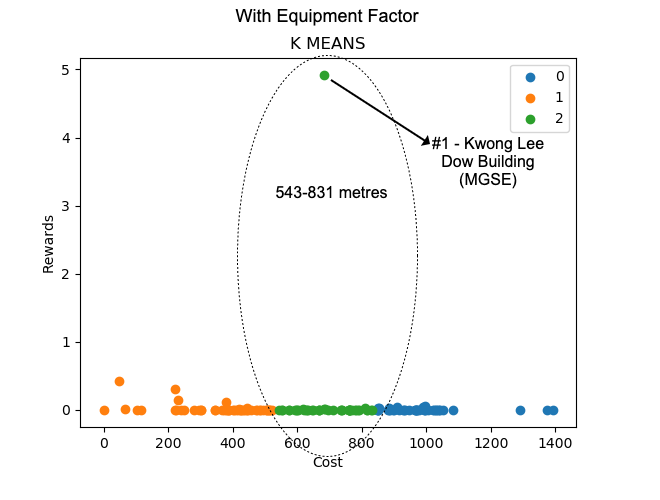
\includegraphics[width=5.5cm,keepaspectratio=true]{resources/images/spatial-mr/barry-mr/11_barry_st_05.png}
% \end{subfigure}
% \begin{subfigure}[b]{0.30\textwidth}
%   \centering
%   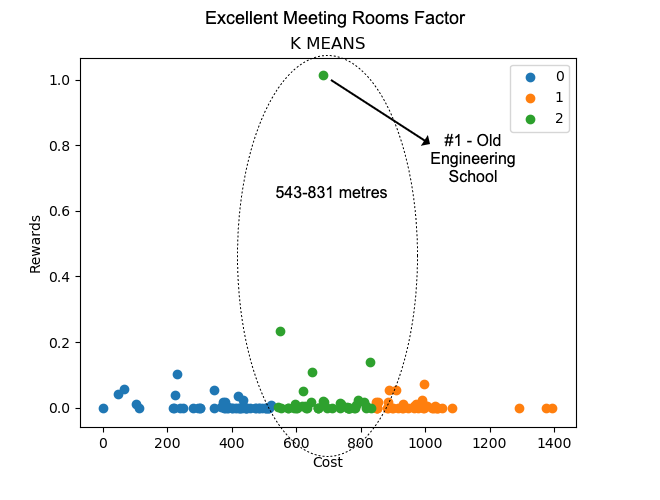
\includegraphics[width=5.5cm,keepaspectratio=true]{resources/images/spatial-mr/barry-mr/11_barry_st_06.png}
% \end{subfigure}
% \caption{Best rewarding clusters of nearby buildings from 11 Barry St based on different factors}
% \label{fig:barry-mr-other-factors}
% \end{figure}

% \paragraph{Law Building (Parkville Campus)}

% \begin{figure}[H]
% \centering
% 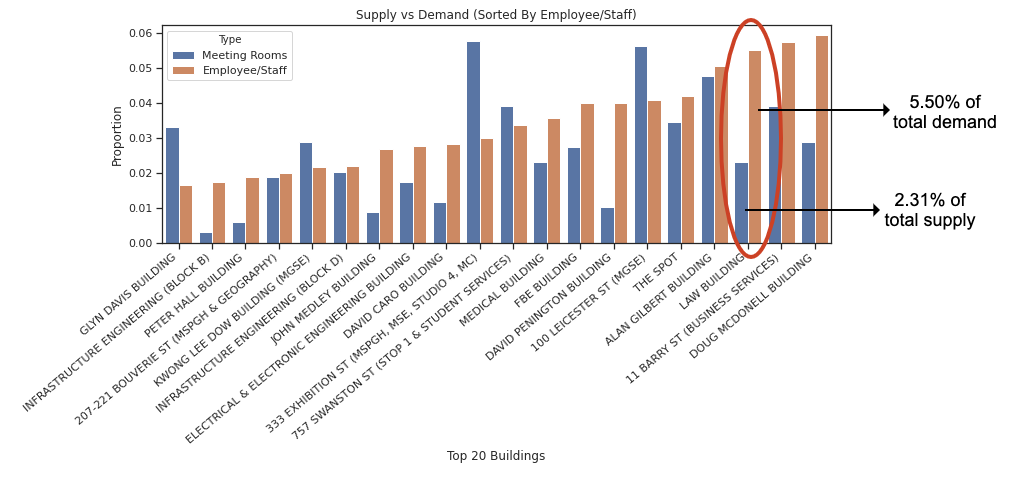
\includegraphics[width=10cm,keepaspectratio=true]{resources/images/spatial-mr/law-mr/law_building_01.png}
% \caption{Supply vs Demand Problem in Law Building}
% \label{fig:law_mr_s_vs_d}
% \end{figure}

% \begin{itemize}
%     \item \textbf{Best nearby buildings with no preference:}
    
%     \begin{figure}[H]
% \begin{subfigure}{.5\textwidth}
% \centering
%   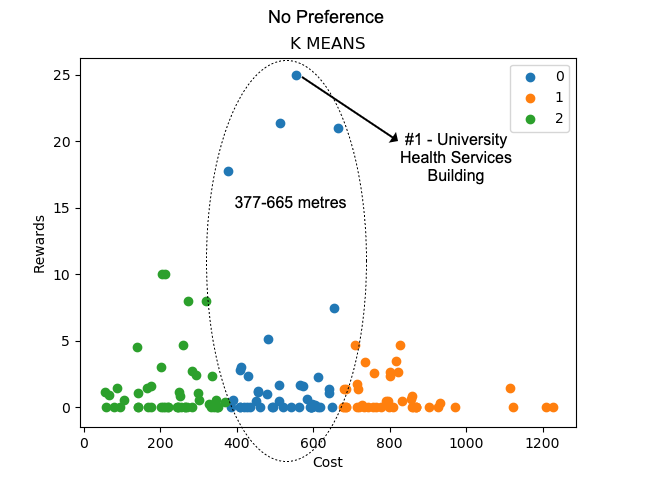
\includegraphics[width=8cm]{resources/images/spatial-mr/law-mr/law_03.png}
% \end{subfigure}%
% \begin{subfigure}{.5\textwidth}
%   \centering
%   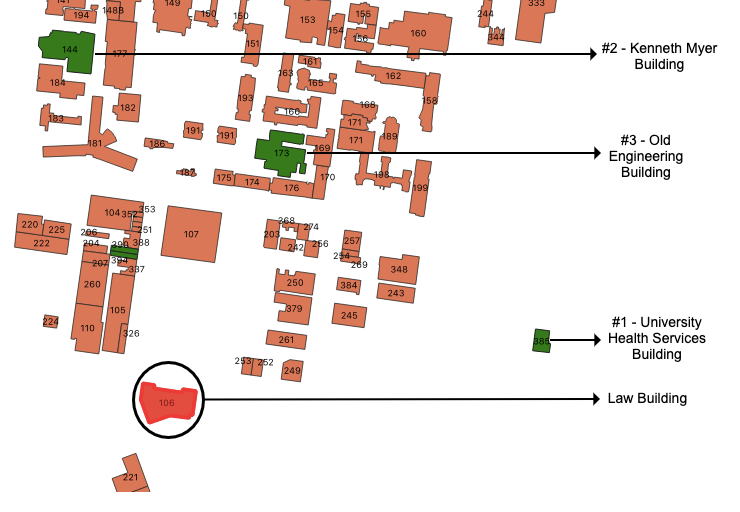
\includegraphics[width=8cm]{resources/images/spatial-mr/law-mr/law_02.png}
% \end{subfigure}
% \caption{Best rewarding cluster (left) and 3 most optimal buildings from Law Building (right)}
% \label{fig:law-mr-no-factors}
% \end{figure}

% \item \textbf{Best nearby buildings with high capacity:}

% \item \textbf{Best nearby buildings with easy availability:}

% \item \textbf{Best nearby buildings with other factors:}

% \end{itemize}

% The results of some of the above discussed factors are summarized below using clustering diagrams.

% \begin{figure}[H]
% \centering
% \begin{subfigure}[b]{0.30\textwidth}
%   \centering
%   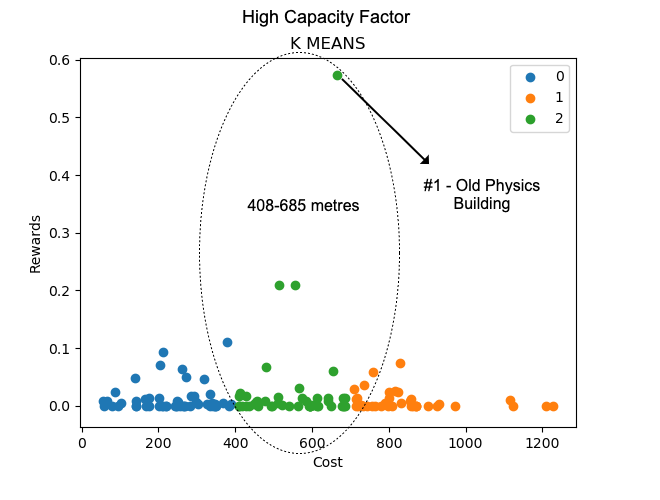
\includegraphics[width=5.5cm,keepaspectratio=true]{resources/images/spatial-mr/law-mr/law_04.png}
% \end{subfigure}
% \begin{subfigure}[b]{0.30\textwidth}
%   \centering
%   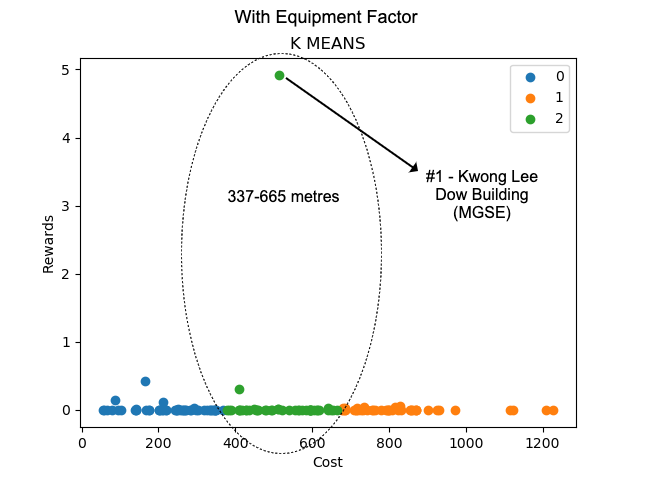
\includegraphics[width=5.5cm,keepaspectratio=true]{resources/images/spatial-mr/law-mr/law_05.png}
% \end{subfigure}
% \begin{subfigure}[b]{0.30\textwidth}
%   \centering
%   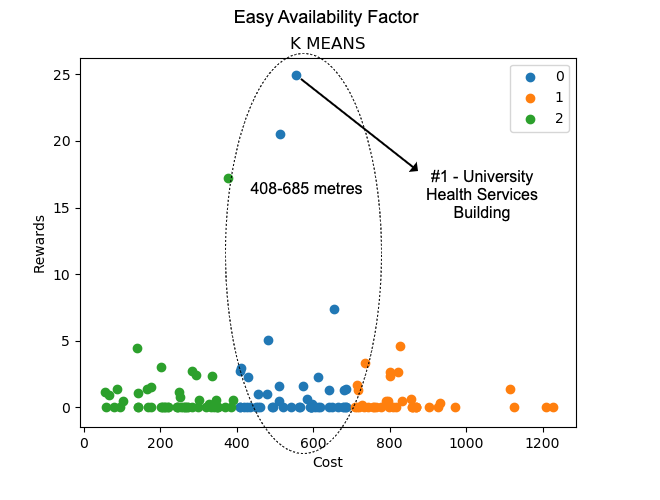
\includegraphics[width=5.5cm,keepaspectratio=true]{resources/images/spatial-mr/law-mr/law_06.png}
% \end{subfigure}
% \caption{Best rewarding clusters of nearby buildings from Law Building based on different factors}
% \label{fig:law-mr-other-factors}
% \end{figure}

\paragraph{David Penington Building (Parkville Campus)}

As per our previous shown data analysis, this building is having a supply-demand problem as shown in the Figure \ref{fig:david_mr_s_vs_d}. 

\begin{figure}[H]
\centering
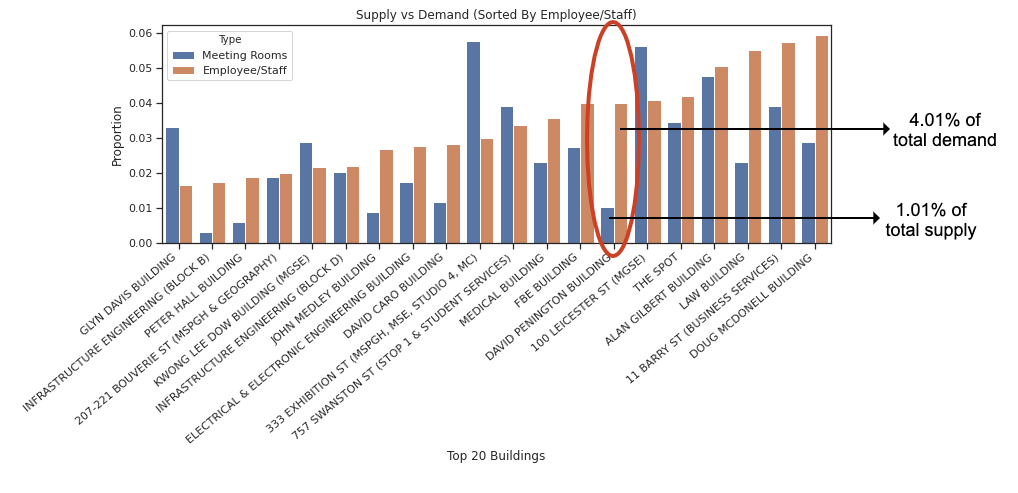
\includegraphics[width=10cm,keepaspectratio=true]{resources/images/spatial-mr/david-mr/david_penington_01.png}
\caption{Supply vs Demand Problem in David Penington Building}
\label{fig:david_mr_s_vs_d}
\end{figure}

% As per the above plot, we can expect that there is a high chance that staff members are not able to find adequate meeting rooms in this building. Hence, we used our algorithm to find other best nearest buildings from David Penington Building based on the different factors as interpreted below.

\begin{itemize}
    \item \textbf{Best nearby buildings with no preference:}
    
    As shown in the Appendix Table \ref{appendix:david_building_mr_table}, a staff member needs to walk at least \texttt{439 metres} (Budget) from David Penington Building to get rewarding buildings with an adequate supply of meeting rooms. We also suggest a relaxing budget ($\delta$) of \texttt{100 metres} so that employee doesn't miss out a high supply providing building. Using these constraints, we suggest \texttt{Kenneth Myer Building (144)} as the most rewarding building with the cost of \texttt{439 metres} as shown in the Figure \ref{fig:david-mr-no-factors}.
    
    \begin{figure}[H]
\begin{subfigure}{.5\textwidth}
\centering
  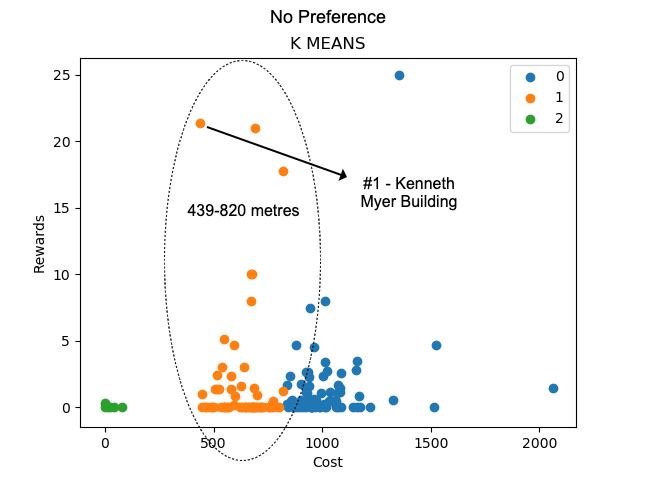
\includegraphics[width=8cm]{resources/images/spatial-mr/david-mr/david_02.png}
\end{subfigure}%
\begin{subfigure}{.5\textwidth}
  \centering
  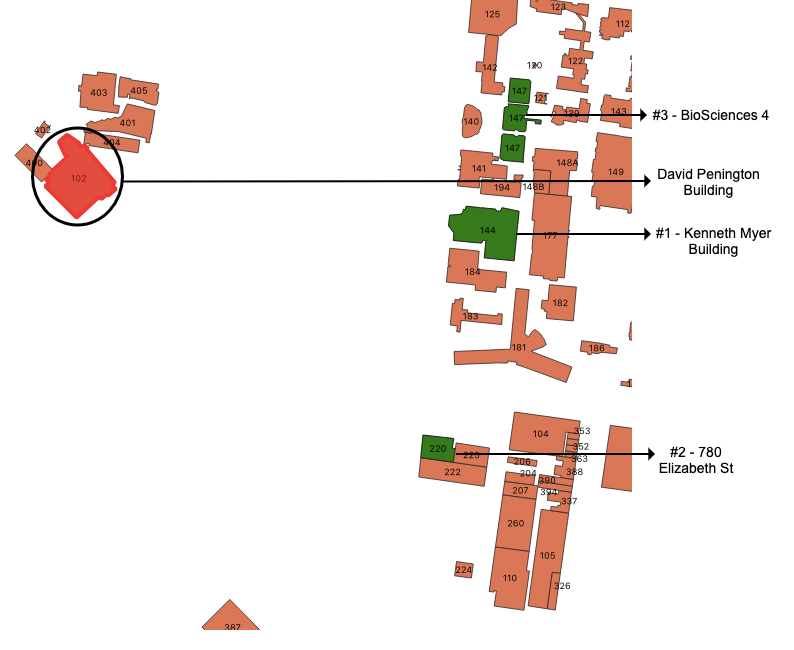
\includegraphics[width=8cm]{resources/images/spatial-mr/david-mr/david_03.png}
\end{subfigure}
\caption{Best rewarding cluster (left) and 3 most optimal buildings from David Penington Building (right)}
\label{fig:david-mr-no-factors}
\end{figure}

% \item \textbf{Best nearby buildings under COVID-19 Strict Lockdown:}

\item \textbf{Best nearby buildings with high capacity:} As shown in the Appendix Table \ref{appendix:david_building_mr_table} with high capacity factor, a staff member can easily find a high supply of meeting rooms providing buildings from David Penington building within the budget of \texttt{690 metres}. Using these constraints, we suggest \texttt{Old Physics Buildings (128)} as the most rewarding building with the cost of \texttt{689 metres} followed by \texttt{Kenneth Myer Building (144)} with \texttt{439 metres} and \texttt{141 Barry St (390)} with \texttt{670 metres}.

\item \textbf{Best nearby buildings with other factors:} In the appendix Table \ref{appendix:doug_mr}, we have also shown other factors such as COVID-19 lockdown, finding meeting rooms with equipment, excellent conditions and easy availability with their budgets and relaxing budgets. Using those constraints, we suggest that \texttt{Kenneth Myer Building (173) - 439 metres} is the most rewarding building for meeting rooms with equipment and finding easily available rooms. \texttt{The Spot Building (385) - 685 metres} is the most rewarding building in the COVID-19 strict lockdown situation.

\end{itemize}

The results of some of the above-discussed factors are summarized below using clustering diagrams.

\begin{figure}[H]
\centering
\begin{subfigure}[b]{0.30\textwidth}
  \centering
  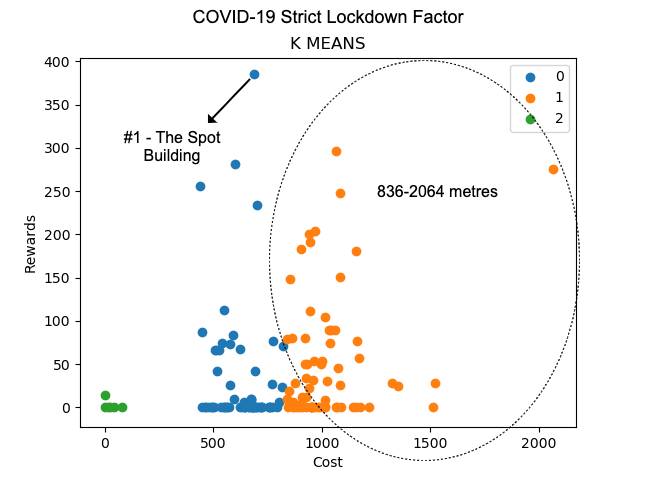
\includegraphics[width=5.5cm,keepaspectratio=true]{resources/images/spatial-mr/david-mr/david_04.png}
\end{subfigure}
\begin{subfigure}[b]{0.30\textwidth}
  \centering
  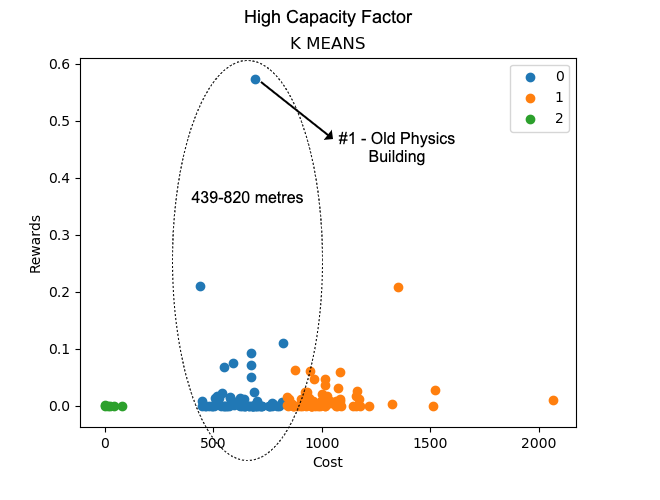
\includegraphics[width=5.5cm,keepaspectratio=true]{resources/images/spatial-mr/david-mr/david_05.png}
\end{subfigure}
\begin{subfigure}[b]{0.30\textwidth}
  \centering
  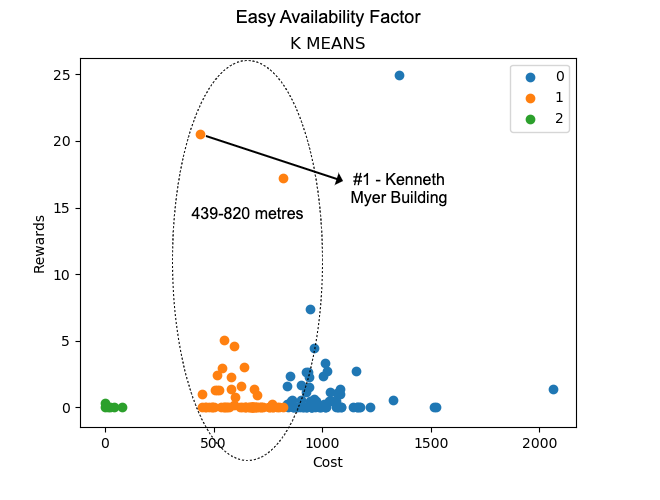
\includegraphics[width=5.5cm,keepaspectratio=true]{resources/images/spatial-mr/david-mr/david_06.png}
\end{subfigure}
\caption{Best rewarding clusters of nearby buildings from David Penington Building based on different factors}
\label{fig:david-mr-other-factors}
\end{figure}

% \paragraph{FBE Building (Parkville Campus)}

% \begin{figure}[H]
% \centering
% 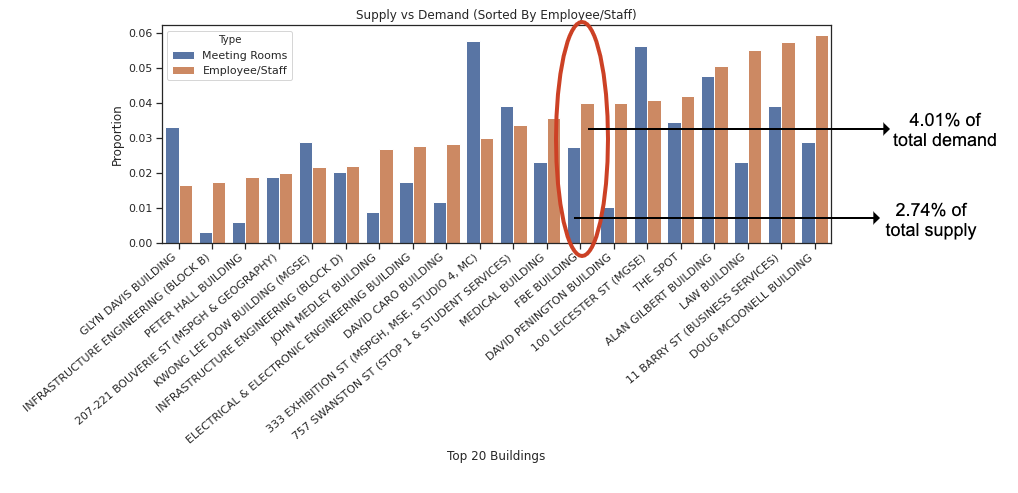
\includegraphics[width=10cm,keepaspectratio=true]{resources/images/spatial-mr/fbe-mr/fbe_building_01.png}
% \caption{Supply vs Demand Problem in FBE Building}
% \label{fig:fbe_mr_s_vs_d}
% \end{figure}

% \begin{itemize}
%     \item \textbf{Best nearby buildings with no preference:}
    
%     \begin{figure}[H]
% \begin{subfigure}{.5\textwidth}
% \centering
%   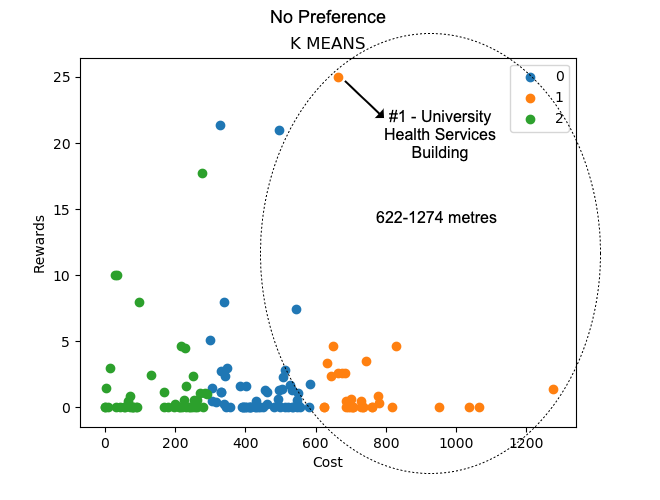
\includegraphics[width=8cm]{resources/images/spatial-mr/fbe-mr/fbe_02.png}
% \end{subfigure}%
% \begin{subfigure}{.5\textwidth}
%   \centering
%   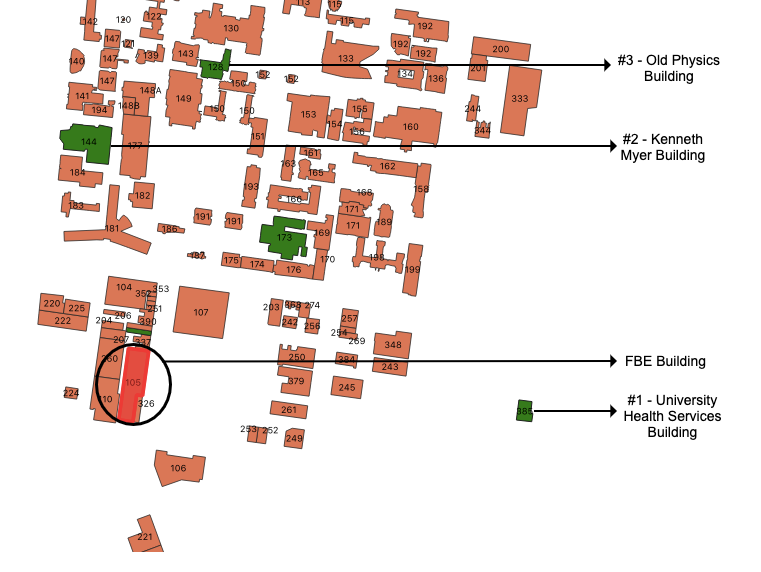
\includegraphics[width=8cm]{resources/images/spatial-mr/fbe-mr/fbe_03.png}
% \end{subfigure}
% \caption{Best rewarding cluster (left) and 3 most optimal buildings from FBE Building (right)}
% \label{fig:fbe-mr-no-factors}
% \end{figure}

% \item \textbf{Best nearby buildings with high capacity:}

% \item \textbf{Best nearby buildings with excellent room conditions:}

% \item \textbf{Best nearby buildings with other factors:}

% \end{itemize}

% The results of some of the above discussed factors are summarized below using clustering diagrams.

% \begin{figure}[H]
% \centering
% \begin{subfigure}[b]{0.30\textwidth}
%   \centering
%   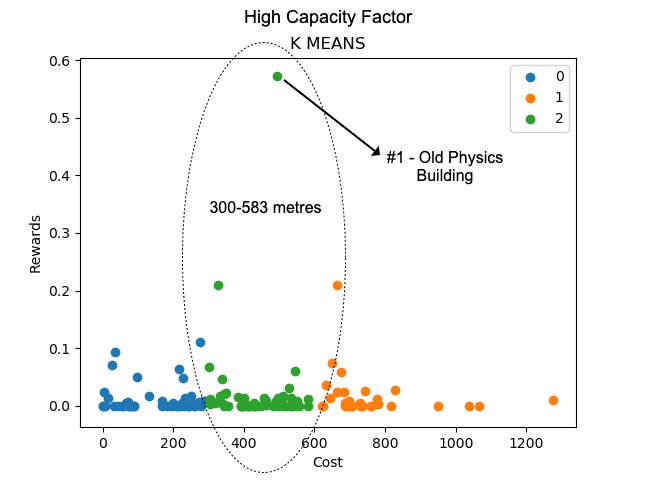
\includegraphics[width=5.5cm,keepaspectratio=true]{resources/images/spatial-mr/fbe-mr/fbe_04.png}
% \end{subfigure}
% \begin{subfigure}[b]{0.30\textwidth}
%   \centering
%   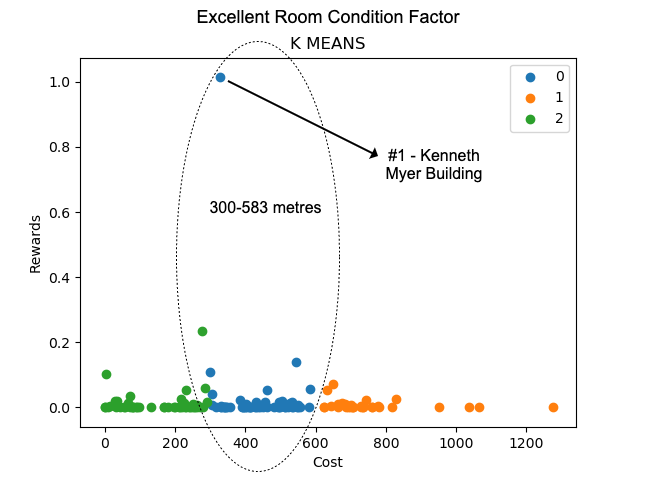
\includegraphics[width=5.5cm,keepaspectratio=true]{resources/images/spatial-mr/fbe-mr/fbe_05.png}
% \end{subfigure}
% \begin{subfigure}[b]{0.30\textwidth}
%   \centering
%   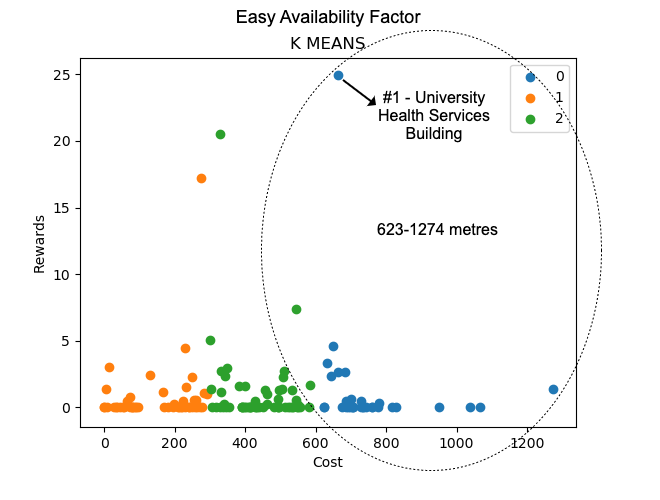
\includegraphics[width=5.5cm,keepaspectratio=true]{resources/images/spatial-mr/fbe-mr/fbe_06.png}
% \end{subfigure}
% \caption{Best rewarding clusters of nearby buildings from FBE Building based on different factors}
% \label{fig:fbe-mr-other-factors}
% \end{figure}

% \paragraph{Medical Building (Parkville Campus)}

% \begin{figure}[H]
% \centering
% 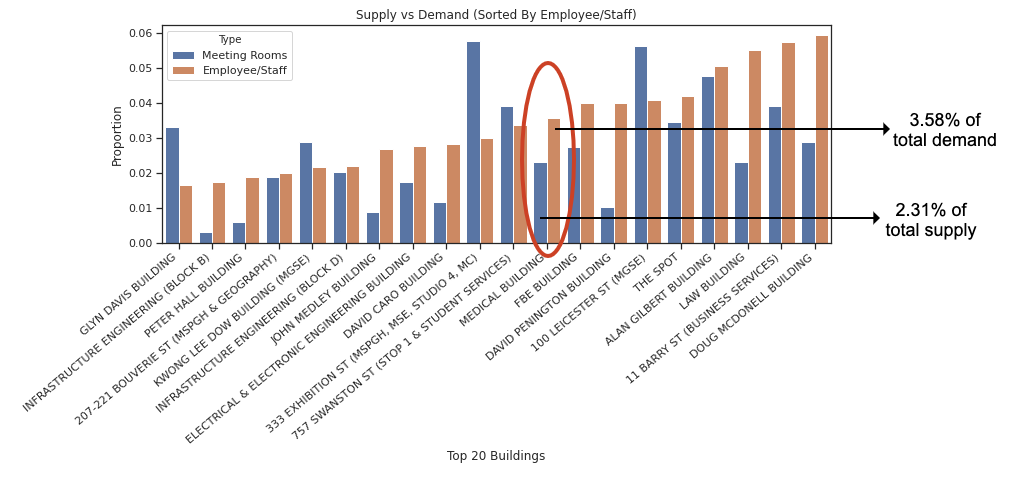
\includegraphics[width=10cm,keepaspectratio=true]{resources/images/spatial-mr/medical-mr/medical_building_01.png}
% \caption{Supply vs Demand Problem in Medical Building}
% \label{fig:medical_mr_s_vs_d}
% \end{figure}

% \begin{itemize}
%     \item \textbf{Best nearby buildings with no preference:}
    
%     \begin{figure}[H]
% \begin{subfigure}{.5\textwidth}
% \centering
%   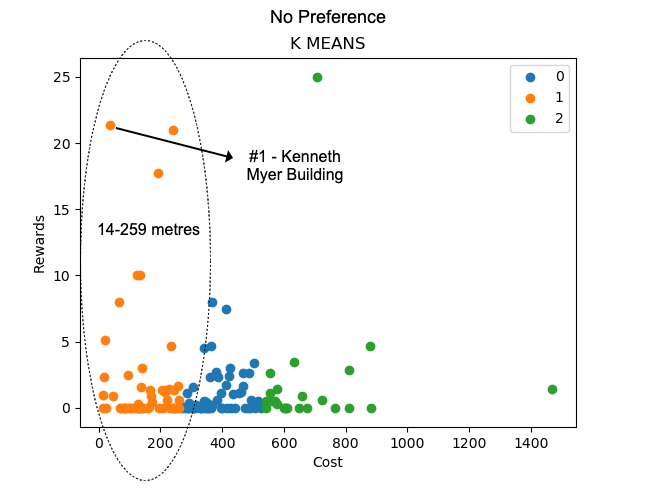
\includegraphics[width=8cm]{resources/images/spatial-mr/medical-mr/medical_02.png}
% \end{subfigure}%
% \begin{subfigure}{.5\textwidth}
%   \centering
%   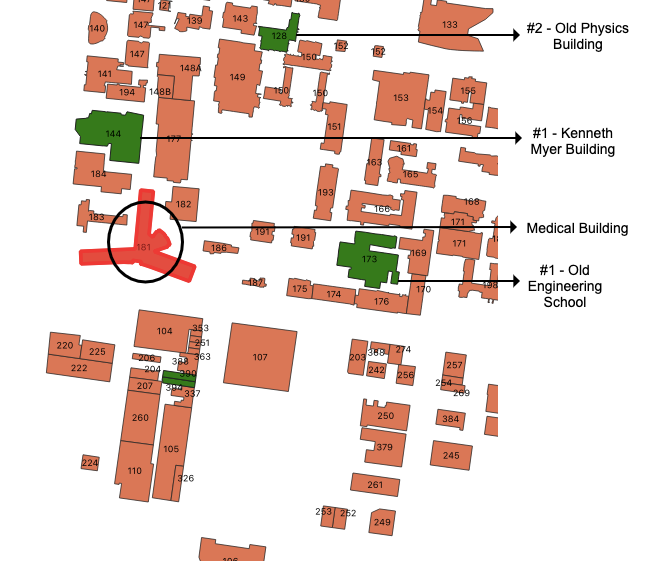
\includegraphics[width=8cm]{resources/images/spatial-mr/medical-mr/medical_03.png}
% \end{subfigure}
% \caption{Best rewarding cluster (left) and 3 most optimal buildings from Medical Building (right)}
% \label{fig:medical-mr-no-factors}
% \end{figure}

% \item \textbf{Best nearby buildings under COVID-19 Strict Lockdown:}

% \item \textbf{Best nearby buildings with high capacity:}

% \item \textbf{Best nearby buildings with other factors:}

% \end{itemize}

% The results of some of the above discussed factors are summarized below using clustering diagrams.

% \begin{figure}[H]
% \centering
% \begin{subfigure}[b]{0.30\textwidth}
%   \centering
%   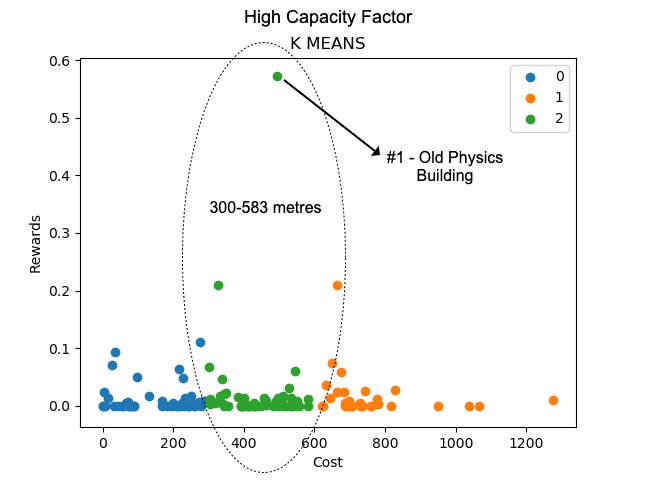
\includegraphics[width=5.5cm,keepaspectratio=true]{resources/images/spatial-mr/fbe-mr/fbe_04.png}
% \end{subfigure}
% \begin{subfigure}[b]{0.30\textwidth}
%   \centering
%   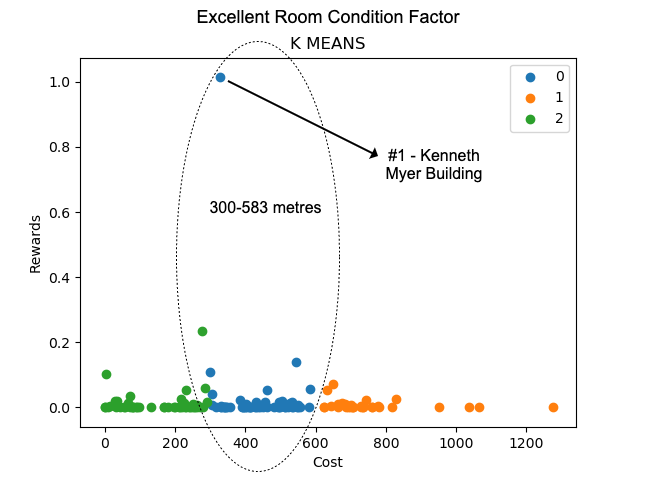
\includegraphics[width=5.5cm,keepaspectratio=true]{resources/images/spatial-mr/fbe-mr/fbe_05.png}
% \end{subfigure}
% \begin{subfigure}[b]{0.30\textwidth}
%   \centering
%   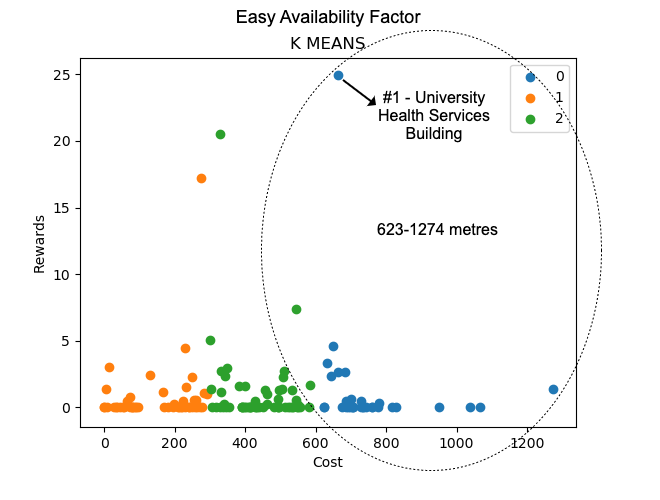
\includegraphics[width=5.5cm,keepaspectratio=true]{resources/images/spatial-mr/fbe-mr/fbe_06.png}
% \end{subfigure}
% \caption{Best rewarding clusters of nearby buildings from FBE Building based on different factors}
% \label{fig:medical-mr-other-factors}
% \end{figure}

\paragraph{Southbank Elisabeth Murdoch Building (Southbank Campus)}

As per our previous shown data analysis, this is another building which is having supply-demand problem as shown in the Figure \ref{fig:southbank_mr_s_vs_d}. 

\begin{figure}[H]
\centering
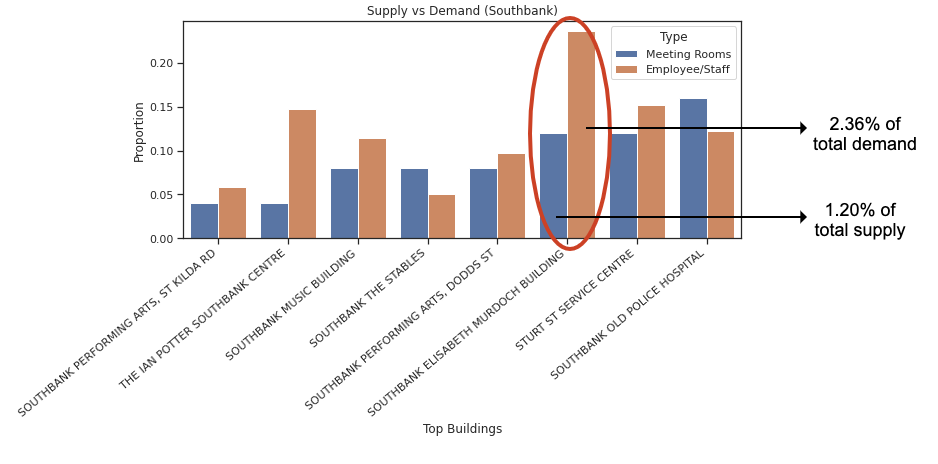
\includegraphics[width=10cm,keepaspectratio=true]{resources/images/spatial-mr/southbank-mr/southbank_01.png}
\caption{Supply vs Demand Problem in Southbank Elisabeth Murdoch Building}
\label{fig:southbank_mr_s_vs_d}
\end{figure}

% As per the above plot, we can expect that there is a high chance that staff members are not able to find adequate meeting rooms in this building. Hence, we used our algorithm to find other best nearest buildings from Elisabeth Murdoch Building based on the different factors as interpreted below.

\begin{itemize}
    \item \textbf{Best nearby buildings with no preference:} As shown in the Appendix Table \ref{appendix:southbank_elisabeth_mr_table}, a staff member needs to walk at least \texttt{130 metres} (Budget) from Elisabeth Murdoch Building to get rewarding buildings with an adequate supply of meeting rooms. Using these constraints, we suggest \texttt{Southbank old police hospital (865)} as the most rewarding building with the cost of \texttt{109 metres} as shown in the Figure \ref{fig:southbank-mr-no-factors}.
    
    \begin{figure}[H]
\begin{subfigure}{.5\textwidth}
\centering
  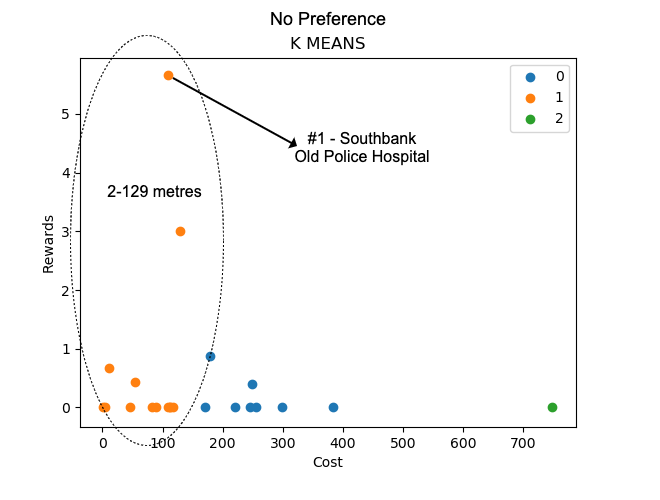
\includegraphics[width=8cm]{resources/images/spatial-mr/southbank-mr/elisabeth_02.png}
\end{subfigure}%
\begin{subfigure}{.5\textwidth}
  \centering
  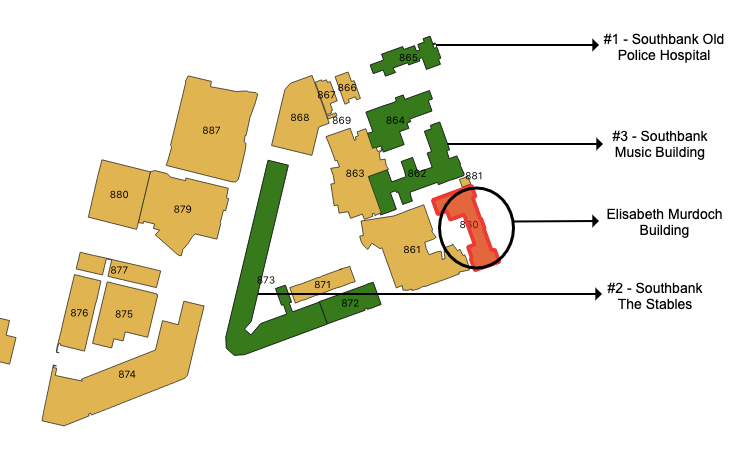
\includegraphics[width=8cm]{resources/images/spatial-mr/southbank-mr/elisabeth_03.png}
\end{subfigure}
\caption{Best rewarding cluster (left) and 3 most optimal buildings from Elisabeth Murdoch Building (right)}
\label{fig:southbank-mr-no-factors}
\end{figure}

\item \textbf{Best nearby buildings under COVID-19 Strict Lockdown:} As shown in the Appendix Table \ref{appendix:southbank_elisabeth_mr_table} with COVID-19 strict factor, a staff member should be willing to walk at least \texttt{130 metres} (Budget) from Elisabeth Murdoch Building to get very high rewarding buildings under COVID-19 lockdown. Using these constraints, we again suggest \texttt{Southbank old police hospital (865)} as the most rewarding building with the cost of \texttt{109 metres} followed by \texttt{Southbank music building (862)} with \texttt{10 metres} cost.

% \item \textbf{Best nearby buildings with high capacity:}

\item \textbf{Best nearby buildings with other factors:} In the appendix Table \ref{appendix:southbank_elisabeth_mr_table}, we have also shown other factors such as finding meeting rooms with equipment, excellent conditions and easy availability with their budgets and relaxing budgets. Using those constraints, we suggest that \texttt{Ian potter Southbank centre (880) - 248 metres} is the most rewarding building for meeting rooms with equipment. \texttt{Southbank old police hospital (865)} remains as the most rewarding building for finding easy available, excellent condition and high capacity meeting rooms.

\end{itemize}

% \paragraph{Werribee Pathology Building (Werribee Campus)}

% \begin{figure}[H]
% \centering
% 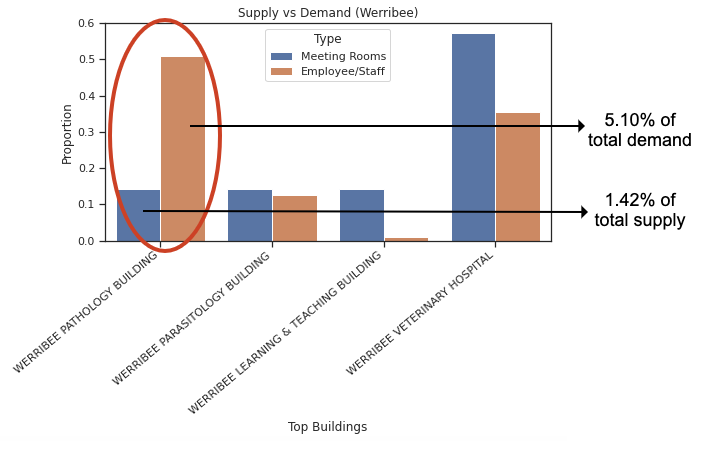
\includegraphics[width=10cm,keepaspectratio=true]{resources/images/spatial-mr/werribee-mr/werribee_01.png}
% \caption{Supply vs Demand Problem in Werribee Pathology Building}
% \label{fig:werribee_mr_s_vs_d}
% \end{figure}




